\documentclass[10pt]{article}
\usepackage{a4wide}
\usepackage[english]{babel}
\usepackage{graphicx}
\usepackage{tabu}
\usepackage{textcomp}
\usepackage{fancyhdr}
\usepackage{lastpage}
\usepackage{titlesec}
\usepackage{lscape}
\usepackage{longtable}
\usepackage{color}
\usepackage{listings}
\usepackage{xkeyval}
\usepackage{hyperref}

\definecolor{mygreen}{rgb}{0,0.6,0}
\definecolor{mygray}{rgb}{0.5,0.5,0.5}
\definecolor{mymauve}{rgb}{0.58,0,0.82}

\lstset{ % Syntax highliughting for java
  backgroundcolor=\color{white},   % choose the background color; you must add \usepackage{color} or \usepackage{xcolor}
  basicstyle=\footnotesize,        % the size of the fonts that are used for the code
  breakatwhitespace=false,         % sets if automatic breaks should only happen at whitespace
  breaklines=true,                 % sets automatic line breaking
  captionpos=b,                    % sets the caption-position to bottom
  commentstyle=\color{mygreen},    % comment style
  deletekeywords={...},            % if you want to delete keywords from the given language
  escapeinside={\%*}{*)},          % if you want to add LaTeX within your code
  extendedchars=true,              % lets you use non-ASCII characters; for 8-bits encodings only, does not work with UTF-8
  frame=none,                    % adds a frame around the code
  keepspaces=true,                 % keeps spaces in text, useful for keeping indentation of code (possibly needs columns=flexible)
  keywordstyle=\color{blue},       % keyword style
  language=Octave,                 % the language of the code
  morekeywords={*,...},            % if you want to add more keywords to the set
  numbers=left,                    % where to put the line-numbers; possible values are (none, left, right)
  numbersep=5pt,                   % how far the line-numbers are from the code
  numberstyle=\tiny\color{mygray}, % the style that is used for the line-numbers
  rulecolor=\color{black},         % if not set, the frame-color may be changed on line-breaks within not-black text (e.g. comments (green here))
  showspaces=false,                % show spaces everywhere adding particular underscores; it overrides 'showstringspaces'
  showstringspaces=false,          % underline spaces within strings only
  showtabs=false,                  % show tabs within strings adding particular underscores
  stepnumber=5,                    % the step between two line-numbers. If it's 1, each line will be numbered
  stringstyle=\color{mymauve},     % string literal style
  tabsize=4,                       % sets default tabsize to 2 spaces
  title=\lstname                   % show the filename of files included with \lstinputlisting; also try caption instead of title
}
%%%%%%
%% Variables for version and release status
%% useage: \version
%%%%%%
\newcommand\module{CS223}
\newcommand\assignmentTitle{North Ceredigion Fitness Website Prototype Development}
\newcommand\authorText{Nicholas Dart}
\newcommand\authorUsername{nid21}
\newcommand\studentID{130057750}
\newcommand\assesser{Angharad Shaw}

%%%%%%
%% Alias
%%%%%%
%\newcommand{\sectionbreak}{\clearpage}    %% Allways start a section on a new page

\title{ \huge \module~Assignment \\ \Large \assignmentTitle}
\author{
  \vspace{100pt}
  \begin{tabular}{ r || l }
    Author          & \authorText (\authorUsername)\\
            & \studentID \\
    Date Published  & \today \\
            & \\
    Assessed By     & \assesser \\
    Department      & Computer Science \\
    Address         & Aberystwyth University \\
            & Penglais Campas \\
            & Ceredigion \\
            & SY23 3DB \\
  \end{tabular} \\
  Copyright \textcopyright~Aberystwyth University 2015
  %get rid of the date on the titlepage
  \date{}
}

\pagestyle{fancy}
\fancyhf{}
\lhead{\module~Assignment}
\rhead{\authorText~-~\studentID}
\rfoot{Page \thepage \hspace{1pt} of \pageref{LastPage}}
\lfoot{Aberystwyth University - Computer Science}

\begin{document}
  \setcounter{page}{1}

  \maketitle
  \thispagestyle{empty}
  \clearpage

  \tableofcontents
  \clearpage

  \section{Introduction}
    For this assignment, I approached it by looking for websites that I felt were good examples of how a site should be laid out, either through how the site is navigated, it's design style, colour theme or other features that lend themselves to the site. 

    \url{https://news.ycombinator.com/}\\
    Hacker news is a very simple yet elegant technology/startup news forum, I consider it a good example as it is a simple design, that very minimal yet still has all the features of a forum such as voting, comments and karma.

    \url{http://google.co.uk}\\
    Google is a nice example as it's style and design haven't changed much over the years; it's kept a relatively consistent style and layout and not cluttered it's interface (such as alternatives like Bing). I prefer designs and UI that are clean and minimal, whilst having features that are needed/relevant in drop down/pull out drawers such as getting to gmail, calendar and drive from google's homepage.
    
    \url{http://imgur.com/}\\
    Imgur is a simple image sharing site. It provides tools for users to upload and share images, as well as commenting on them. It has a minimal style, however provides tools such as view/comment/point statistics on images, as well as allowing the user to choose how they view the content (grid, list, slideshow, etc). It also integrated with other content forms such as gifs and galaries of multiple images within the same layout, allowing for an easier viewing experience. 

  \section{Task Analysis}
    Some functional requirements were provided in the assignment brief; however I have expanded these here (for later reference) and in the use case diagram\ref{fig:usecase};

    \begin{description}
      \item[FR1] The administrator should be able to:
      \begin{description}
        \item[FR1.1] Create entries for new classes
        \item[FR1.2] Delete classes
        \item[FR1.3] Change time of classes
        \item[FR1.4] Create new instructor accounts
        \item[FR1.5] Set venue for classes
      \end{description}
      \item[FR2] An instructor should be able to:
      \begin{description}
        \item[FR2.1] Cancel individual classes and give reason
        \item[FR2.2] Temporary change class times
        \item[FR2.3] Post notices about classes
        \item[FR2.4] Post attendance information
        \item[FR2.5] View attendance information
      \end{description}
      \item[FR3] Subscribed Members should be able to:
      \begin{description}
        \item[FR3.1] Subscribe to classes
        \item[FR3.2] Subscribe from classes
      \end{description}
      \item[FR4] Member of public should be able to:
      \begin{description}
        \item[FR4.1] View class times
        \item[FR4.2] View class venue
        \item[FR4.3] View class instructor
        \item[FR4.4] View class notices
      \end{description}
    \end{description}

    In the above analysis, I have assumed that a user type (ie ``Subscribed Member'') also has the task requirements of the previous one (ie ``Member of public''). Except for an instructors and administrators, who I assume cannot subscribe to a class.

    The requirement specification also described examples of special cases for class scheduling;
    \begin{verbatim}
...to take account of term times (e.g. Thursdays 15th January-26th March AND
16th April-25th June at 7 pm).
    \end{verbatim}

    This I have assumed is done by postponing or adding class times as needed for set durations.

    \begin{figure}[p]
      \centering
      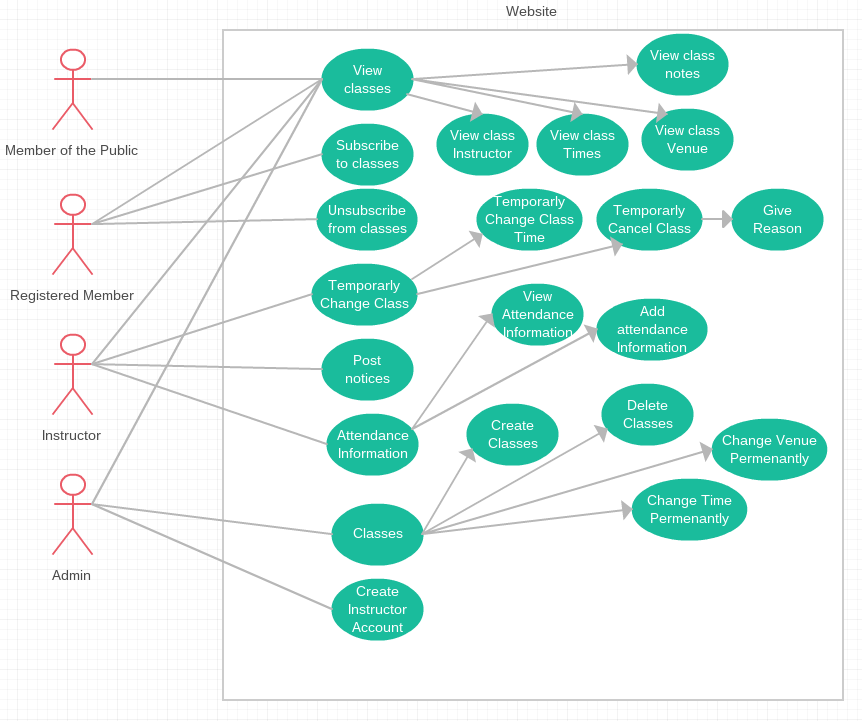
\includegraphics[width=1\textwidth]{usecasediagram.png}
      \caption{Use case Diagram for the system}
      \label{fig:usecase}
    \end{figure}

    \section{A high level design of interaction, navigation and overall layouts}
      Initial design brainstorming was done with Cormac Brady (cob16), Owen Garland (owg1) and Xander Barnes (acb12), we brainstormed ideas for design, user flow and layout ideas, however we did not design a site, merely discuss our ideas and opinions. \ref{fig:plan}

      \begin{figure}[p]
        \centering
        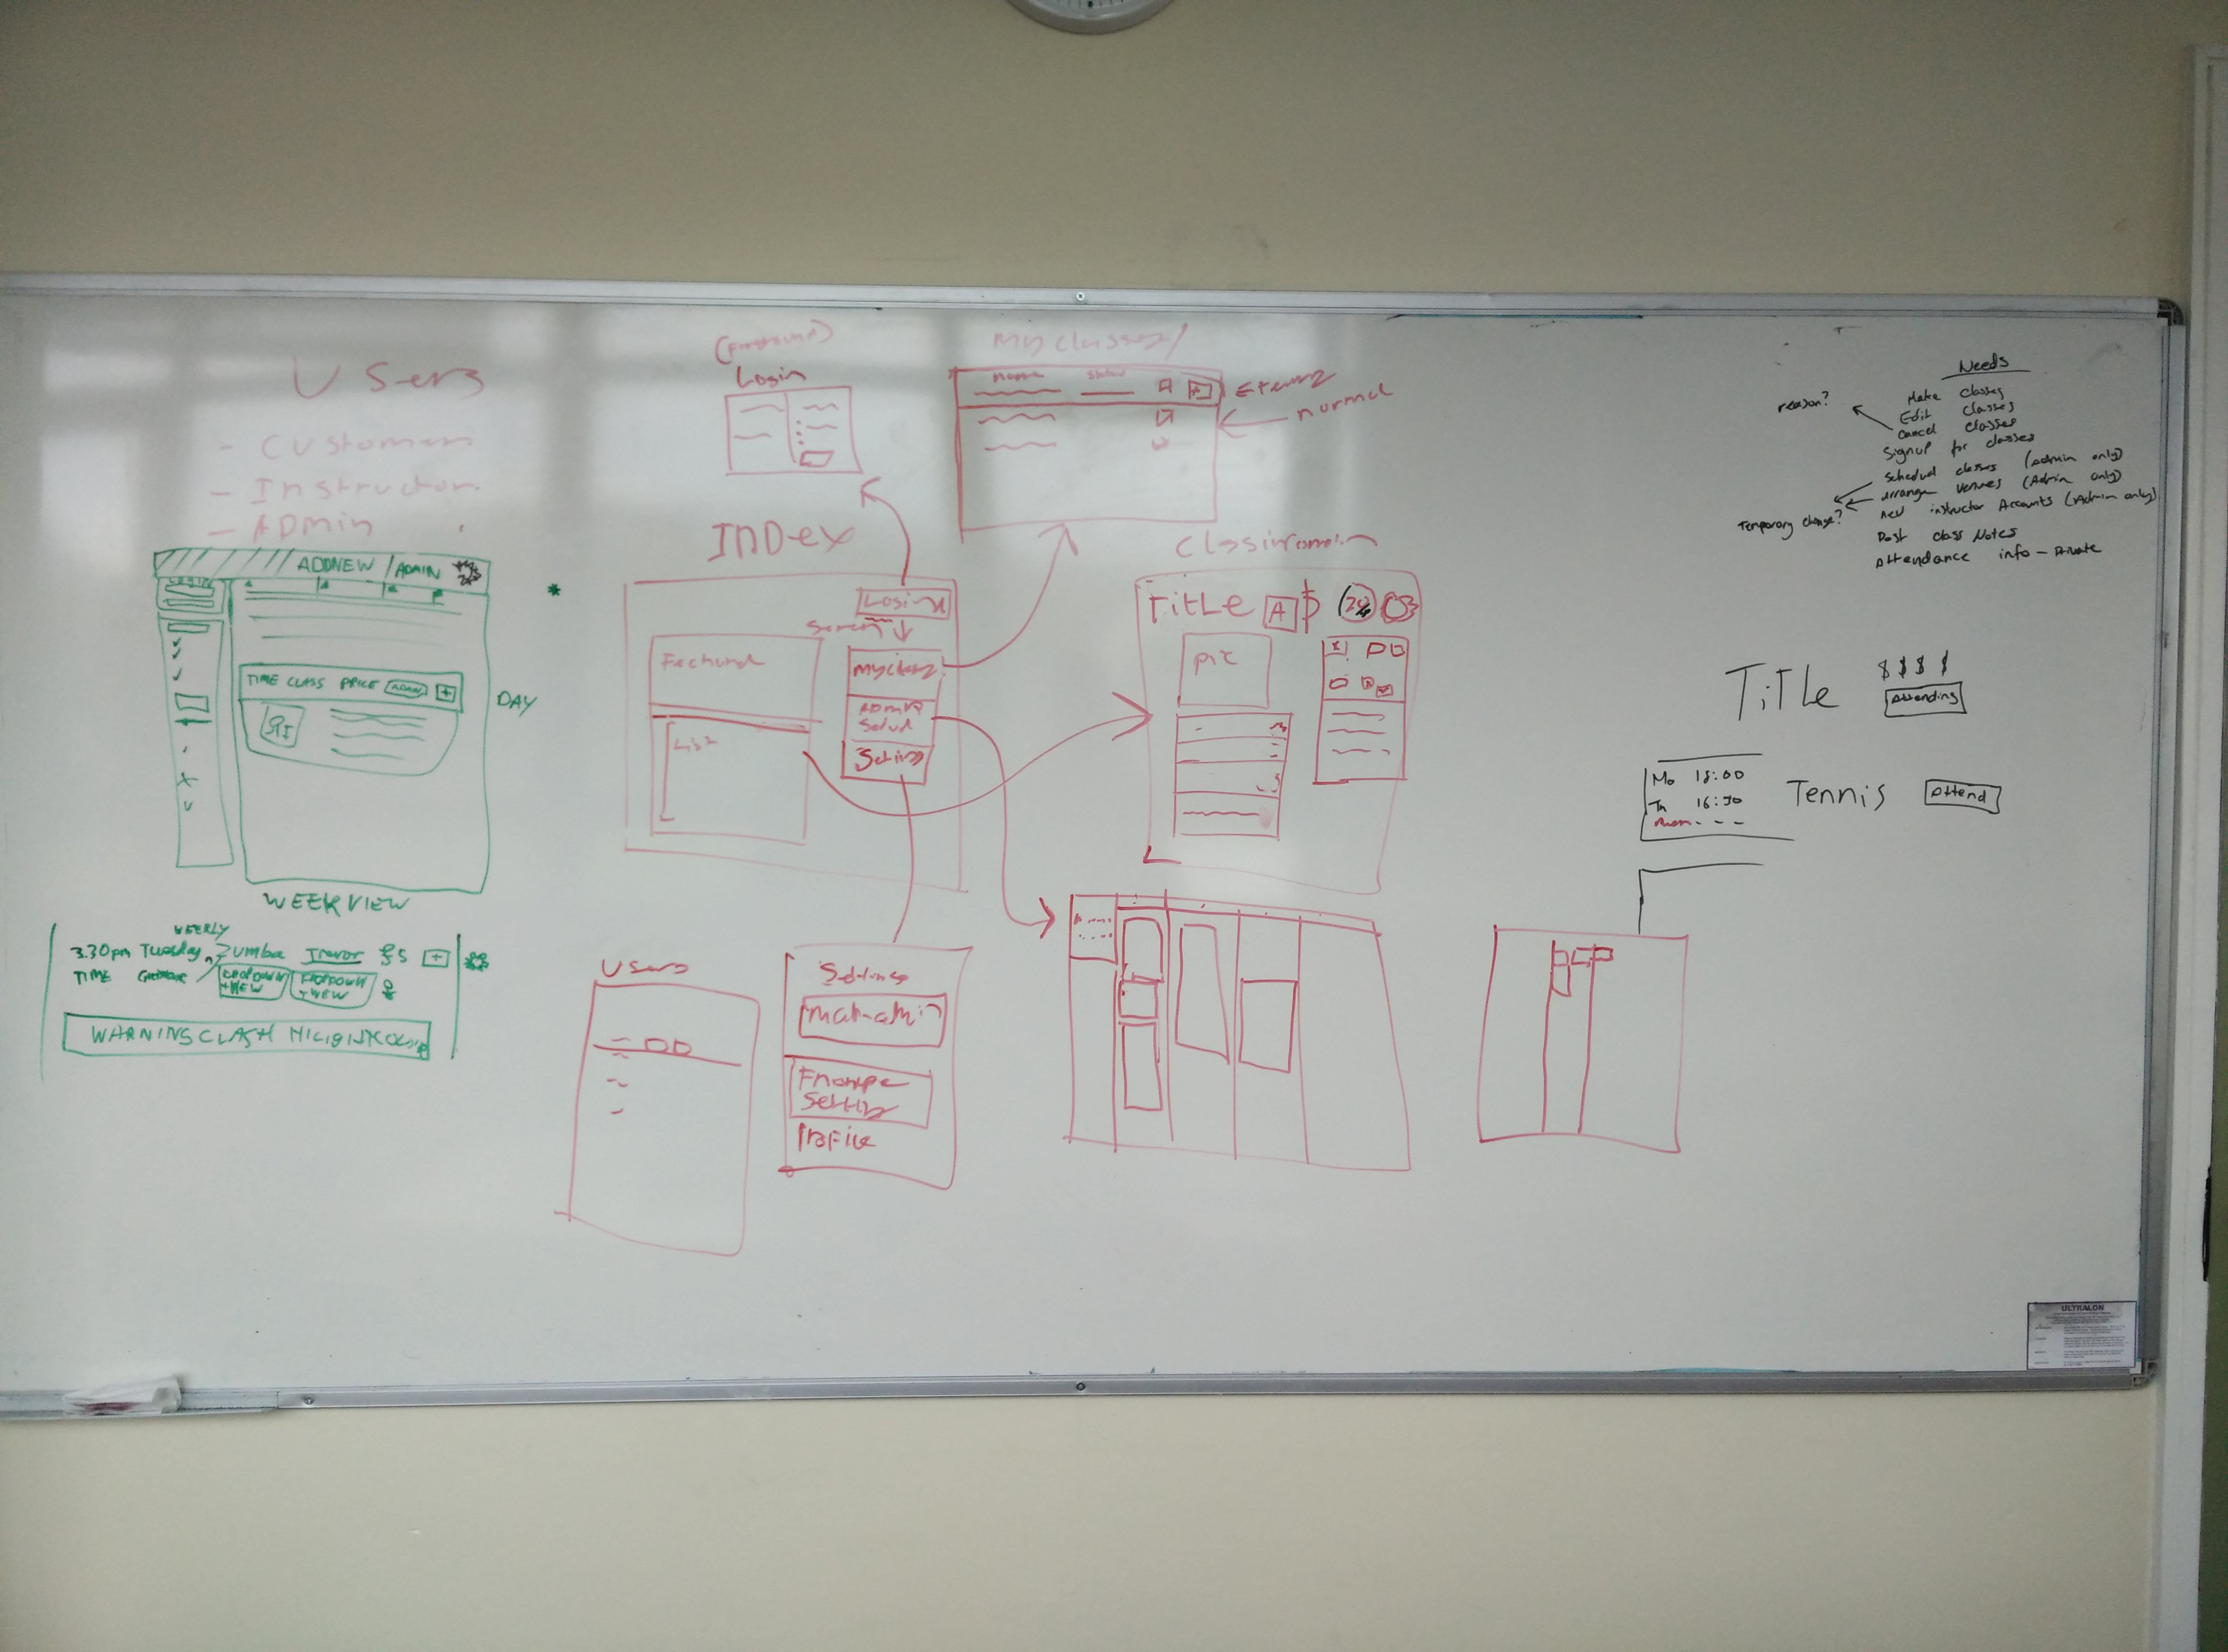
\includegraphics[width=1\textwidth]{prototype.jpg}
        \caption{Initial planning on a whiteboard}
        \label{fig:plan}
      \end{figure}

      For the design of the site, I have decided to use twitter's bootstrap front end framework; it allows for fast prototyping and a consistent look, as well as being responsive and mobile friendly. It also has support for screen readers through use of labels, help text and semantic markup (by way of use of html5).\cite{bootstrapScreenReader} For the site, as the majority of users visiting it being people browsing for classes or people subscribing to classes, I believe that a single page interface should suffice as no new content will be being created by them. Similarly for an instructor, they are not creating much content, simply editing the class description, postponing or cancelling classes with optional reasoning. They can also most likely suffice with a single page. 

      I have chosen this root of a single page as it can streamline the experience, with Ajax being used functionally to pull data when needed. It should also give a seamless experience for the user, being able to subscribe to multiple classes quickly with a single click without having to wait for a page to reload to continue their work. The user, however should be presented with a confirmation after subscribing to a class, for example the subscribe button should change to a loading or processing animation when clicked and then be replaced with a red/warning coloured subscribe button when they have been successfully subscribed. This gives them feedback that they have been subscribed successful, without resetting the page or interrupting their work flow. In the event of an error, a popup dialogue should be presented with a suitable error message and description as to what the user did wrong and what they can do to fix it; eg ``The class is now full, please choose another day or time'', or who to contact if it is a more serious problem eg ``Your card was not processed correctly, please email support@domain.com to arrange alternate payment or try again later''.

      I also plan to have a choice of layouts, a list based layout where users can choose first the type of activity they want (eg ``Rock Climbing'') then the type they want, this process will allow for a more concise list of activities, hopefully reducing the need to scroll through large numbers of pages of repeating information. It should also give the user confidence that if a time is not listed under a sport that is convenient for them, then such a time does not exist, allowing for a faster viewing and decision process. In addition to the list based layout, a grid layout that provides all the previous information but in a grid based layout for more condensed information as well as possible pictures of the sport or activity. This grid should also contain only a single tile for a sport or activity and should open to reveal all the times for that sport, again to help speed up the browsing process. Finally a calendar option should be made available where logged in users can view the times of classes they've subscribed to.

      Instructors, who I have treated as a privileged user, are afforded a very similar interface albeit with the options to alter information on the page. This should help the instructors visualise how the information they choose will be presented the the real user. 

      
      Following Shneiderman’s first, third and sixth rules; a consistent feel, look and operation, offering informative feedback and easy reversal of mistakes, I believe will offer a speedy and simple experience for most users.

      \subsection{Overarching Layout}
        The overall design, which I plan on following on all pages, is as follows;

        At the top, there should be a title, with spaces for pictures, artwork, contact details etc. Directly under this to the left, there should be a user box with details about who is logged in (if applicable) and logout and settings buttons. Under this, but still within the side bar should be any search and layout tools to help the user navigate the class list. There may also be information here to allow for creation of a calendar that the user can add to their personal calendars. Finally, if the user logged in is the administrator, the side bar should also relevant to their work, but not to an individual class. This sidebar, which I am assuming is all one block, should follow the user as they scroll through the page.

        To the right of the side bar, and taking up the rest of the screen realestate, should be the main body of the page. This is where the user can interact with classes. At the top of this main body notifications should be displayed such that they are obvious and prominent when the page is loaded. This main section is where most of the changed between the different types of users occur. There should be a list of classes, which contain the name of the class, instructor and short hand location of the lesson. Clicking on the tab should expand the class to show a list of times, prices and any notes about the class. Any cancellation of classes should be highlighted here with a ``expected next date'' to give users an idea when the service may return. There should also be a map to allow users easy rought finding through a map service, as well as a full address and parking descriptions. Finally there should also be a description of the class provided by the instructors.

      \subsection{Unauthenticated User}
        Unauthenticated users will be shown a simple view of the site, with no ability to subscribe to classes, they will however be presented with a login and register option to allow them to do so. They will be able to view a complete set of classes, class notes and times. This class information will be located in the main body of the page, organised by class name. They will also have access to a filter panel on the left, where they can select a time range for classes to appear in, an option to hide empty and full classes and search by name. 

        The login and register dialogue should be at the top of the main page, such that it is an obvious part of the process in registering, but not obscure the rest of the page such that users might think that they have to register before they can see classes on offer.

      \subsection{Authenticated User}
        Once a user is authenticated, they are presented with an additional filter type; to view classes they are enrolled in. This should hide any classes they have not subscribed to, however if they have subscribed to a class, it should still show all the times available in that class, to allow switching of attended time with ease.

        The side bar should also show the user's information, which may be linked to a profile management system or social media of their choice. As well as having a logout button and a button to change settings and cancel their membership with the fitness group. Finally the side panel should also contain a link to their calendar view, which is personalised to them. There may also be an optional calendar link they may add to their private calendars.

      \subsection{Instructors}
        Instructors should be able to edit information about a activity, namely the description and any specific class notes. The activity description should be a lengthy text piece describing the likely events of the courses and possibly a description of the instructor. They also need to be able to postpone a class, with an optional reason. As this is a task that will effect many people, and requires additional information to complete, a popup or modal dialogue should be used to allow for a reason to be entered and to give the user a chance to undo their actions. 
        
        Finally the instructor should be able to reschedule a class or classes, this is also a task that will effect many users so again a modal should be used.

      \subsection{Administrator}
        The administrator will be required to create new classes, and fill them out. To achieve this a list of classes should be present with an add button at the top to allow for easy addition of classes. When a new class is being created, they should be able to select or create a venue from the list, this new venue should include a brief name and full address, as well as parking information. The creating of new venues should be done in a modal window to allow for creation whist a class is also being created, so that both tasks can be done as one. The instructor should, whist creating a new class or editing an existing one, create a new instructor, similarly in a modal window to allow for a seamless creation experience. The admin should also be able to edit information in an existing class, by simply selecting the class they wish to edit and having the information displayed in relevant edit boxes and drop downs. 

        Finally the admin should also be able to add new instructors outside of a new class creation, via the side menu. This allows for instructors to be created ahead of time that could either be for substitution if needed.

    \section{A high-fidelity prototype implementation of the interface}

      \subsection{Hosting}
        
        The prototype is hosted at 
        \begin{center}
          \url{http://users.aber.ac.uk/nid21/cs223/}
        \end{center}
        With a backup provided at
        \begin{center}
          \url{http://nic-dart.co.uk/~nic/cs223/index.html}
        \end{center}
        And a copy tar'd in \texttt{/aber/nid21/Documents/cs223Backup.tar.gz} on central

      \subsection{Unimplemented Features and Problems}
        \begin{itemize}
          \item The design only provides a list layout for users to view, due to time constraints.
          \item Settings menu for users is non-existent
          \item The ability to look forward or back at class times is non-existent
          \item Instructor and Venue creation modal windows
          \item 
        \end{itemize}
    
    \section{An evaluation of the prototype against Shneiderman’s 8 golden rules}
      \subsection{1. Strive for consistency}
        I feel the design I have created has a very clear style and design, whist also achieving all the necessary goals. Information is presented to the user in a consistent way and format, and allows for easy navigation.

      \subsection{2. Enable frequent users to use shortcuts}
        Whilst no short cut keys were included in the prototype, they could considerably be implemented in the site-proper. I however do feel that user interactions with the site have been minimised by the hierarchical nature of the layout, as well as search features and planning options to help the user narrow down searches and queries. 

      \subsection{3. Offer informative feedback}
        Whist I feel dialogs and popups should be reserved for warnings, errors and dangerous actions (such as deleting, rescheduling, cancelling a class), I feel the site offers informative feedback where appropriate, for example the subscribe button should change from ``Subscribe'' to ``subscribe'' on completion of successful subscription to a class. Information concerning a user directly, such as a class they attend being cancelled, is also presented at the top of the page where they can take note of it quickly without having to search for it. 

      \subsection{4. Design dialogue to yield closure}
        Actions in the site, such as subscribing to a class at a given time, have been grouped together to allow, for example, someone who wishes to participate in a single sport frequently to select multiple times with ease, without being stopped by a confirmation dialogue. Similarly adding new classes by the administrator can be done entirely from the new class dialogue, including creating a new instructor and adding a new venue.

      \subsection{5. Offer simple error handling}
        Whilst no error dialogues were included in the assignment, I feel error dialogues should be kept to a minimal. The user should be alerted when a function or feature failed to work as a direct result of their actions, however in the event of a system failure (eg a service is down), the user should be presented with an inline dialogue informing them, and advising of features they cannot use, but allowing them to continue working as usual. For errors where the user is responsible, a workaround or alternative should be presented eg ``The class is now full, please choose another day or time''. As the site does not have any payment or transaction system incorporated into it, the likelihood of serious errors is limited, however more permanent tasks such as deleting a class or user should and are highlighted with a confirmation dialogue allowing the user to confirm their action.

      \subsection{6. Permit easy reversal of actions}
        Reversal of tasks is allowed largely through contextual changes to inputs, such as a ``Subscribe'' button changing to say ``Unsubscribe'', in this case there is no penalty to subscribing or subscribing as the feature is used to gauge attendance to classes, not make monetary transactions. However with more important tasks such as creating instructor accounts, a dialogue should be presented at the top warning or informing the user of their actions and allowing an easy alternative to undo their actions. 

      \subsection{7. Support internal locus of control}
        The site provides initiative ways for users, especially administrators, to go about their work. For administrators, the use of inline creation tools such as that of the venue and instructor, provide a more streamlined and easy.

      \subsection{8. Reduce short-term memory load}
        As I am a firm believer in minimal and simple, the site was designed to make information readily available in an initiative way, finding a class at a given time is simply a case of selecting the class and then looking at the listed times. Tools for searching have also been included, but not (in my opinion) overdone; a user can tweak the times they are free, hide and show full and empty classes and view their subscribed classes all from the sidebar. 

    \begin{thebibliography}{9}
      \bibitem{bootstrapScreenReader}
        \url{http://getbootstrap.com/css/#forms-help-text}
    \end{thebibliography}
\end{document}
